\documentclass[12pt,a4paper]{article}  % шаблон для статьи, шрифт 12 пт
\usepackage[utf8x]{inputenc}  % использование кодировки Юникод UTF-8
\usepackage[russian]{babel}  % пакет поддержки русского языка
\usepackage{lipsum}  % Рыба-текст
\usepackage[compact]{titlesec}  % для titlespacing
\titlespacing*{\section}{0.75cm}{1em}{0.1em}  % отступ заголовка 
% \titlespacing{\заголовок}{слева}{перед}{после}[справа]
\titlespacing*{\subsection}{0.75cm}{1em}{0.1em}
\usepackage{indentfirst}  % отступ первого абзаца
\setlength{\parindent}{0.75cm}
\usepackage[labelsep=endash]{caption}  % тире вместо двоеточия в картинках
\usepackage{graphicx}  % кртинки
\usepackage{comment}  % комментарии
\usepackage{tabularx}  % таблицы
\usepackage{color}  % цветной код
\usepackage{listings}  % листинги кода из файлов
\usepackage{cite}  % ???
\lstset{ %
	language=C++,                   % выбор языка для подсветки (здесь это С++)
	basicstyle=\small,              % размер и начертание шрифта для подсветки кода
	numbers=left,                   % где поставить нумерацию строк (слева\справа)
	numberstyle=\tiny,              % размер шрифта для номеров строк
	stepnumber=1,                   % размер шага между двумя номерами строк
	numbersep=5pt,                  % как далеко отстоят номера строк от подсвечиваемого кода
	backgroundcolor=\color{white},  % цвет фона подсветки - используем \usepackage{color}
	showspaces=false,               % показывать или нет пробелы специальными отступами
	showstringspaces=false,         % показывать или нет пробелы в строках
	showtabs=false,                 % показывать или нет табуляцию в строках
	frame=false,                    % рисовать рамку вокруг кода
	tabsize=2,                      % размер табуляции по умолчанию равен 2 пробелам
	captionpos=t,                   % позиция заголовка вверху [t] или внизу [b] 
	breaklines=true,                % автоматически переносить строки (да\нет)
	breakatwhitespace=false,        % переносить строки только если есть пробел
	escapeinside={\%*}{*)}          % если нужно добавить комментарии в коде
}

\usepackage{amsmath}
\usepackage{amssymb}
%перенос строк внутри таблиц
\newcommand{\specialcell}[2][c]{%
	\begin{tabular}[#1]{@{}c@{}}#2\end{tabular}}

% нумерация рисунков по номеру главы (e.g. 1.1) для отчёта по курсовой
% \renewcommand\thefigure{\arabic{section}.\arabic{figure}}

% Шаблон создания картинки
% \begin{figure}[hpt!]
% 	\centering
% 	\includegraphics[width=0.6\linewidth]{photo/photo1}
% 	\caption{Подпись к рисунку}
% 	\label{имя ссылки на рисунок}
% \end{figure}

\begin{document}
	
	\thispagestyle{empty}
	
	\begin{center}
		\Large{
			\textbf{МИНОБРНАУКИ РОССИИ}
			
			\textbf{Санкт-Петербургский государственный}
			
			\textbf{электротехнический университет «ЛЭТИ»}
			
			\textbf{им. В.И. Ульянова (Ленина)}
			
			\textbf{Кафедра Физики}
		}
	\end{center}
	
	\topskip=0pt
	\vspace*{\fill}
	\begin{center}
		\Large{
			\textbf{
				Решения задач ИДЗ №1\\
				по дисциплине «Физика»\\
			}
		}
	\end{center}
	\vspace*{\fill}
	
	\begin{tabular}{lcr}
		Студент гр. 9892 & \begin{tabular}{p{60mm}} \\ \hline \end{tabular} & Лескин К.А.  \\\\
		\\\\
		Преподаватель    & \begin{tabular}{p{60mm}} \\ \hline \end{tabular} & Чурганова С.С. 
		\\\\
	\end{tabular} 
	
	\begin{center}
		Санкт-Петербург\\
		2020
	\end{center}
	%////////////////////////////////////////////////////////////////////////////////////////////////
	%////////////////////////////////////////////////////////////////////////////////////////////////
	%////////////////////////////////////////////////////////////////////////////////////////////////
	\newpage
	
	\section*{Условия задач}
	
	\begin{figure}[hpt!]
		\centering
	 	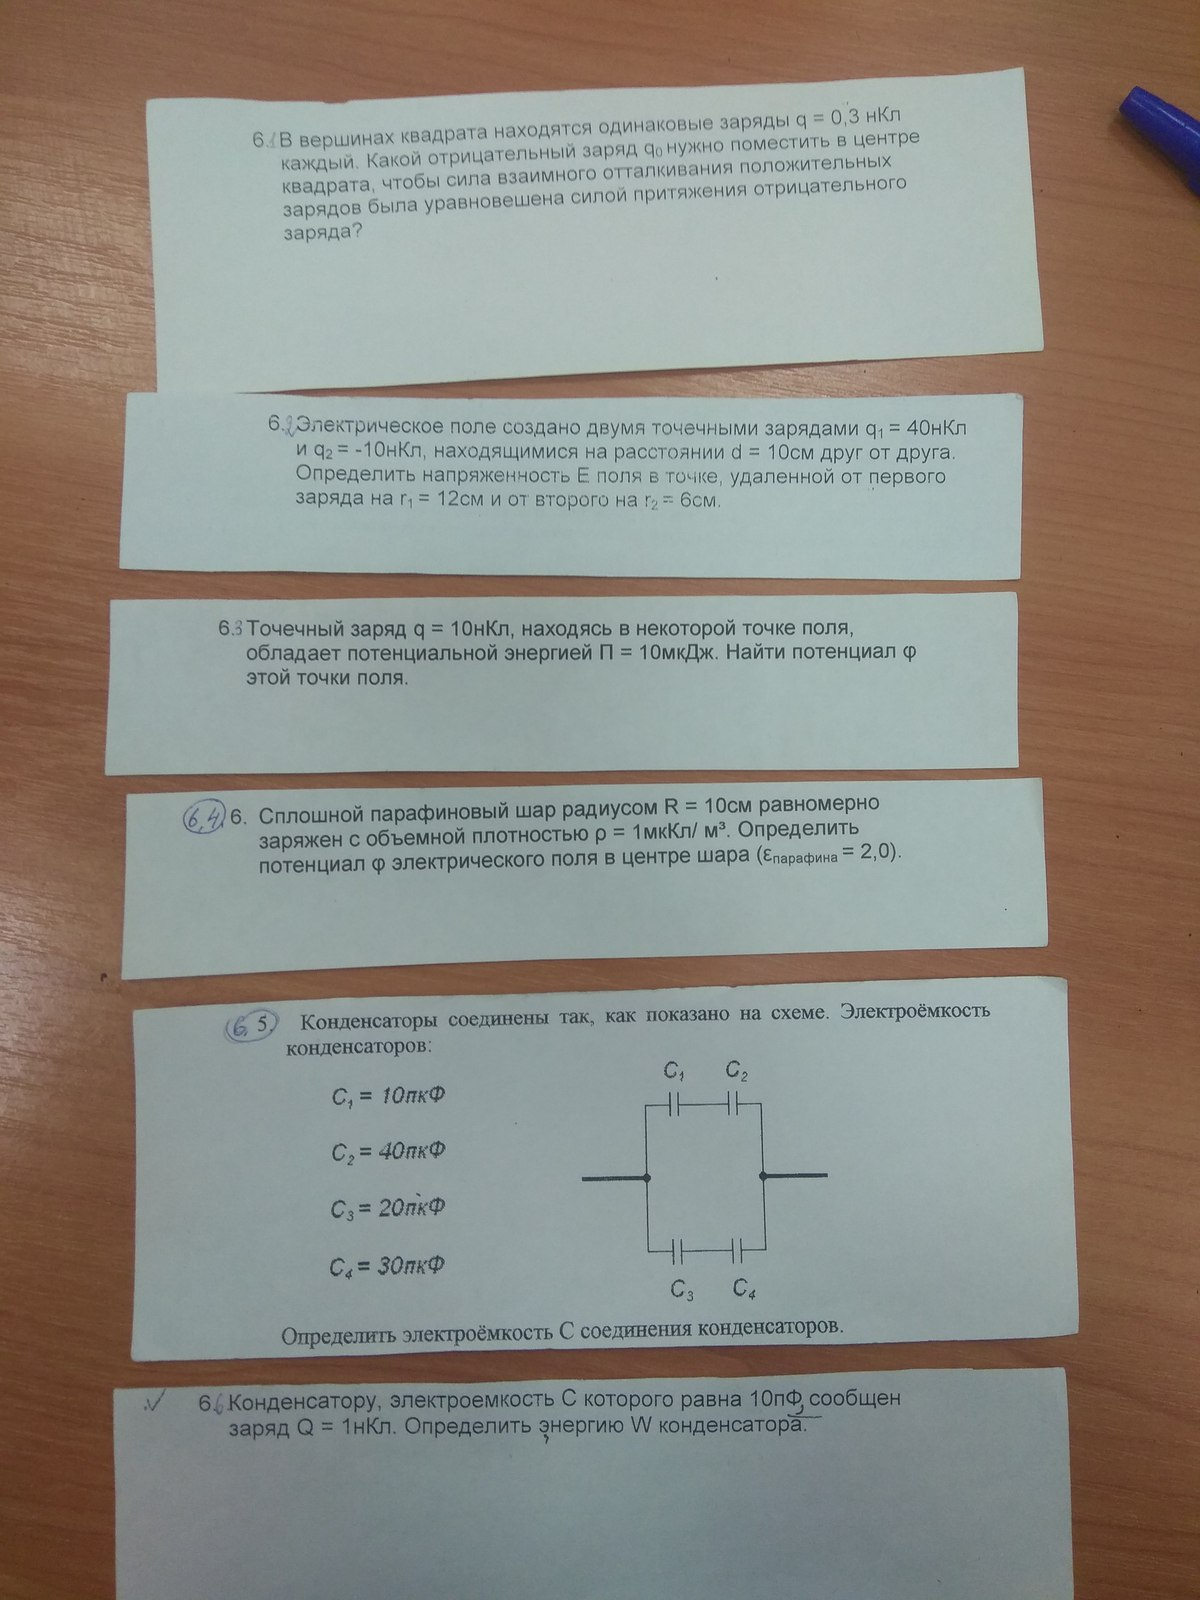
\includegraphics[width=1\linewidth]{photo/tasks_description}
	 	\caption{Условия задач}
	 	\label{tasks}
	\end{figure}

	\section*{Задача 1}
		
	\begin{figure}[hpt!]
		\centering
		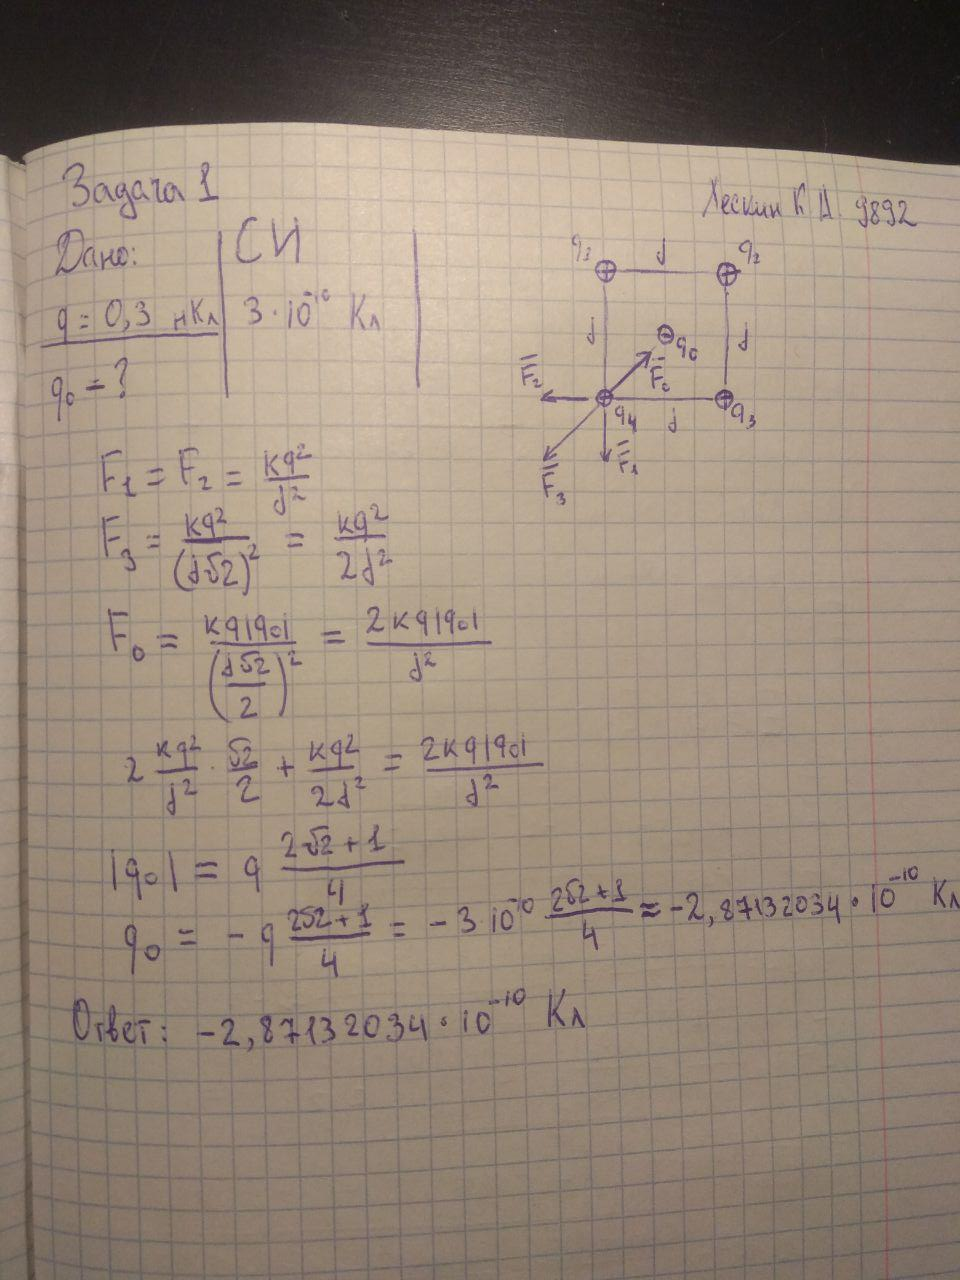
\includegraphics[width=1\linewidth]{photo/task1_solution}
	\end{figure}
	
	\section*{Задача 2}
	
	\begin{figure}[hpt!]
		\centering
		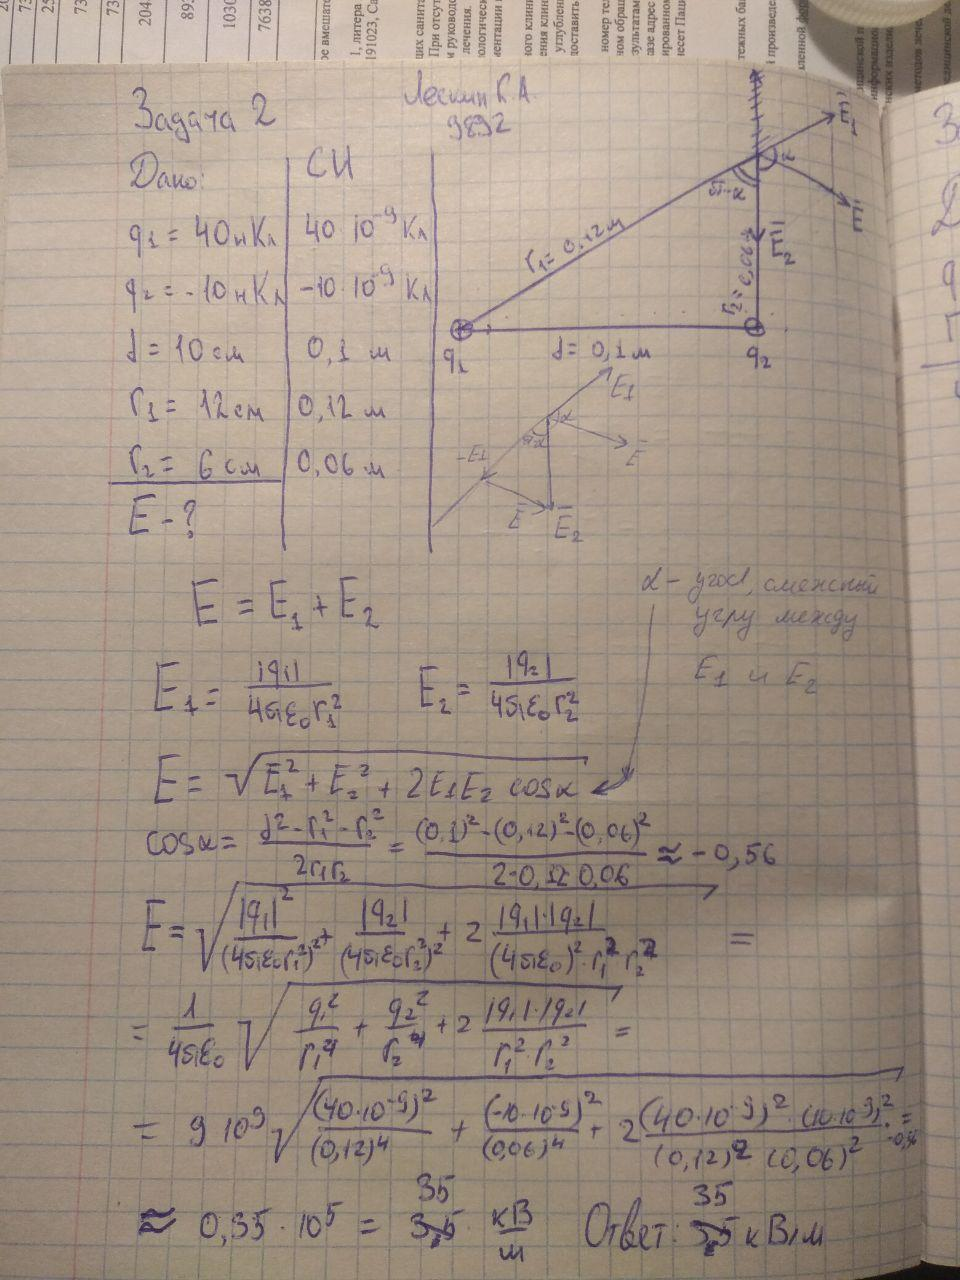
\includegraphics[width=1\linewidth]{photo/task2_solution_update_30_09}
	\end{figure}
	
	\section*{Задача 3}
	
	\begin{figure}[hpt!]
		\centering
		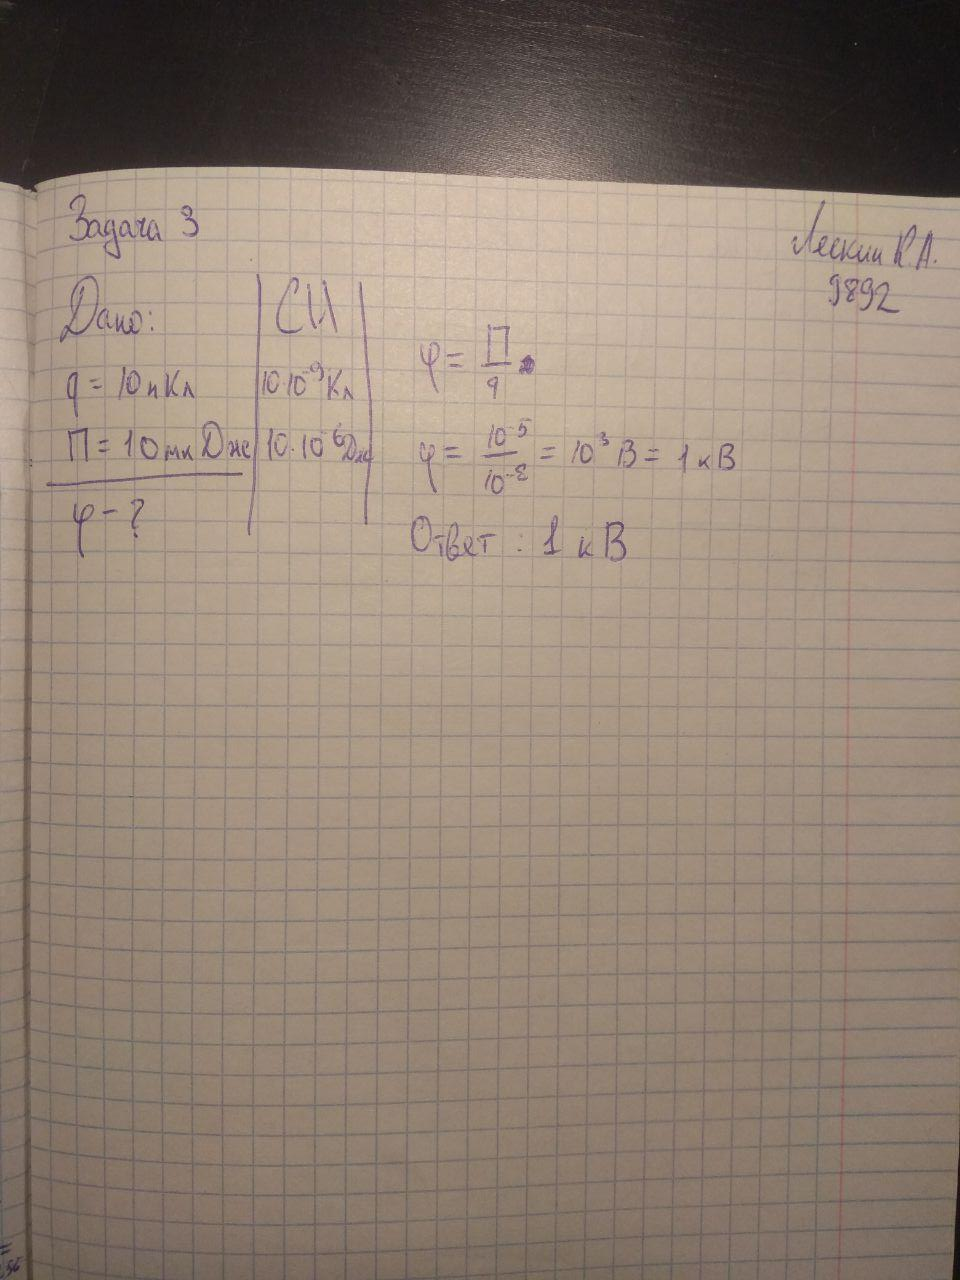
\includegraphics[width=1\linewidth]{photo/task3_solution}
	\end{figure}
	
	\section*{Задача 4}
	
	\begin{figure}[hpt!]
		\centering
		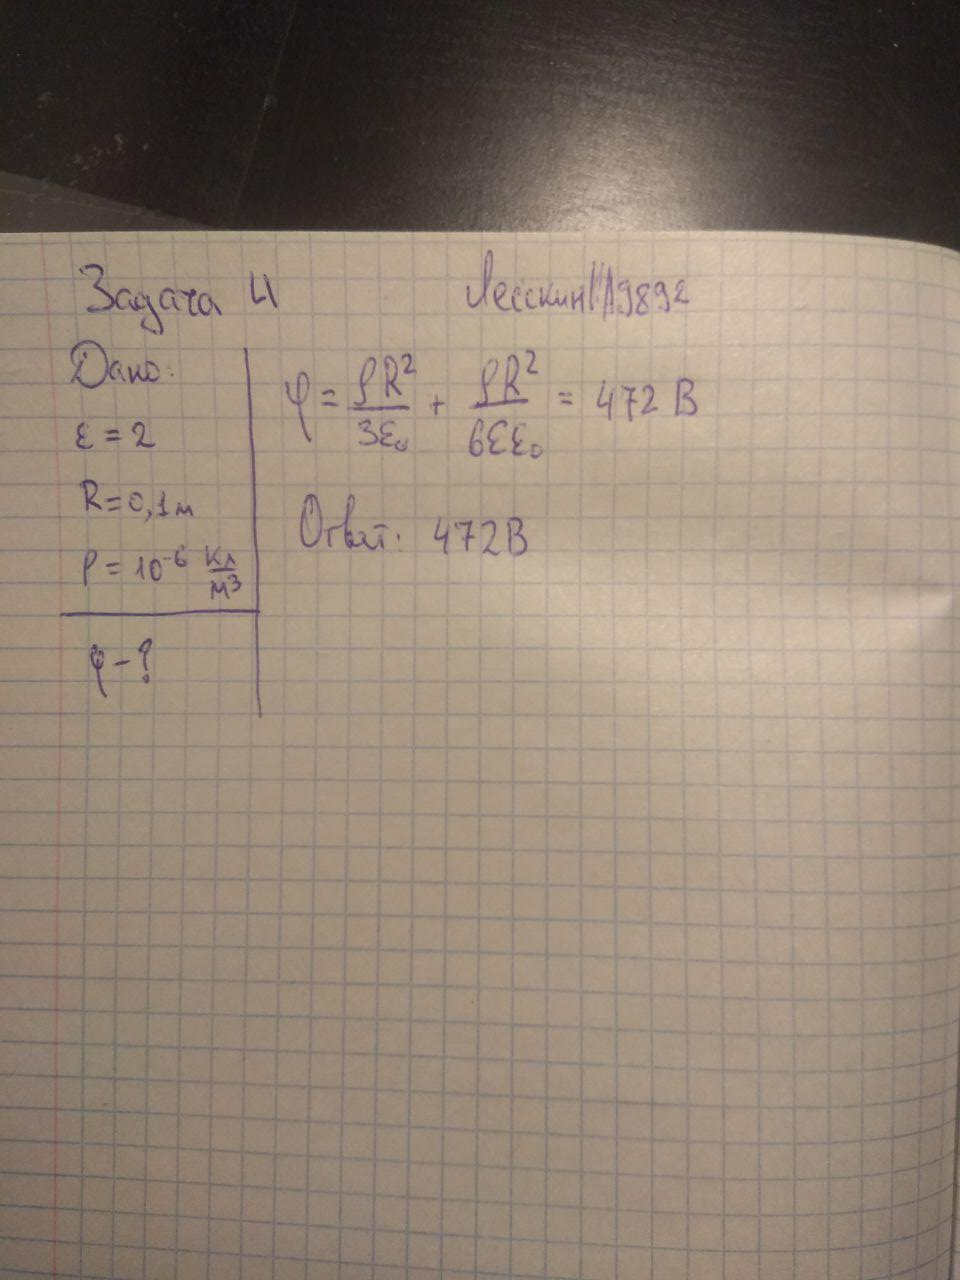
\includegraphics[width=1\linewidth]{photo/task4_solution}
	\end{figure}
	
	\section*{Задача 5}
	
	\begin{figure}[hpt!]
		\centering
		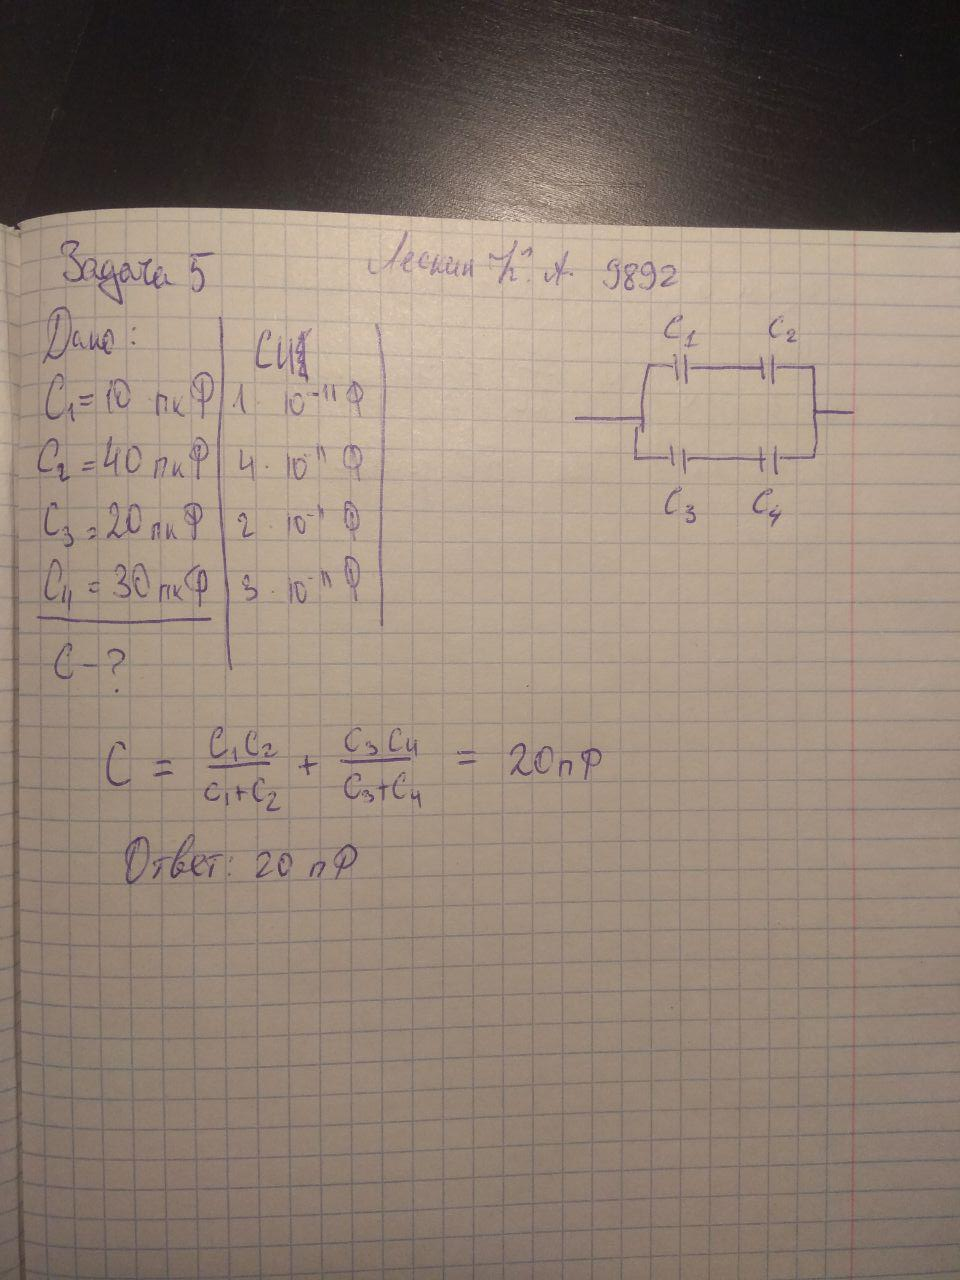
\includegraphics[width=1\linewidth]{photo/task5_solution}
	\end{figure}
	
	\section*{Задача 6}
	
	\begin{figure}[hpt!]
		\centering
		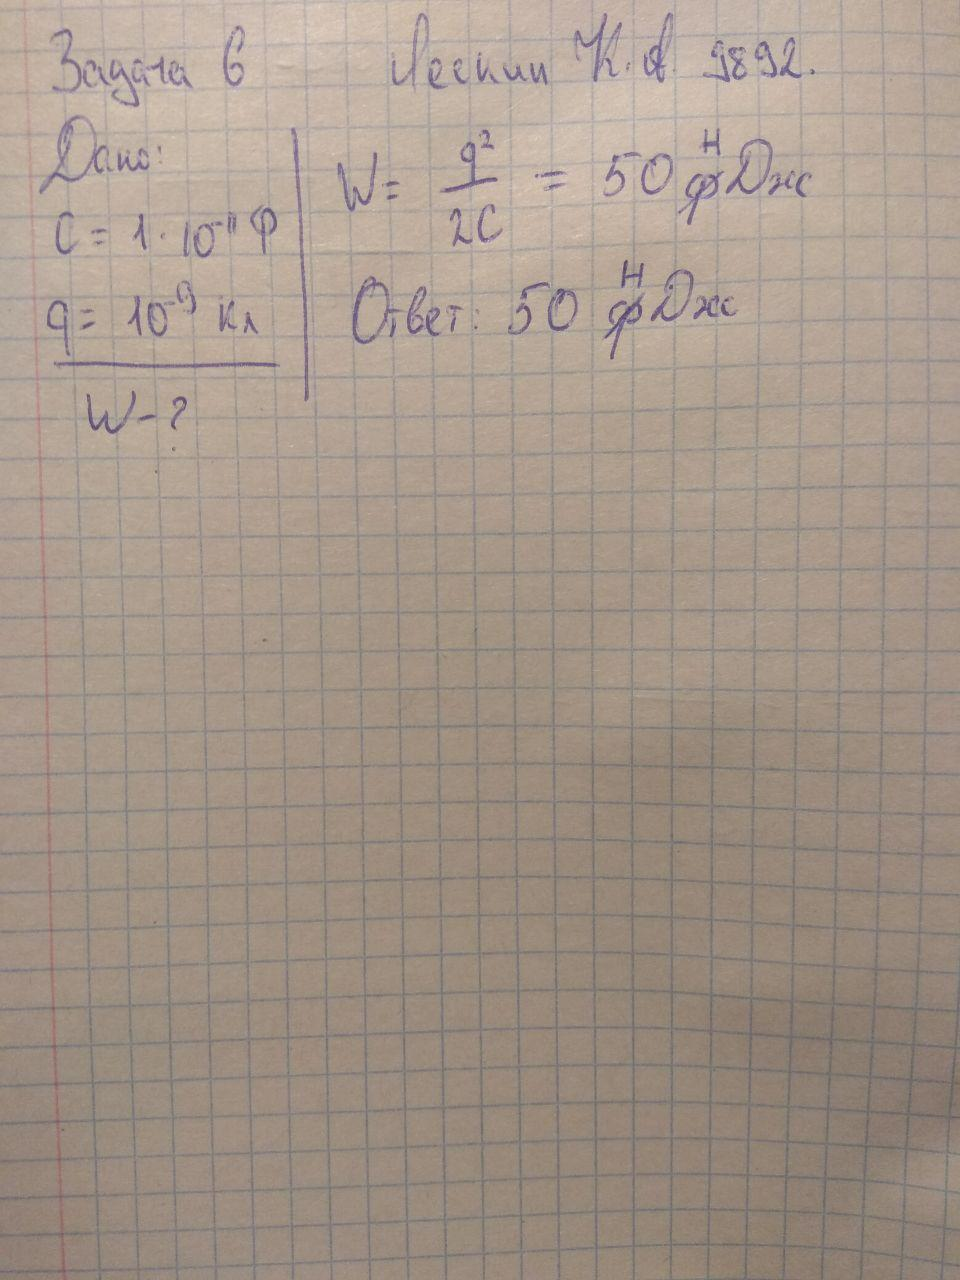
\includegraphics[width=1\linewidth]{photo/task6_solution_update_30_09}
	\end{figure}

	
\end{document}